\documentclass[12pt]{report}

\usepackage[a4paper,
            bindingoffset=0.5cm,
            left=2.5cm,
            right=2.5cm,
            top=5cm,
            bottom=5cm]{geometry}

\usepackage[english]{babel}
\usepackage{amsfonts}
\usepackage{titlesec}
\usepackage{hyperref}
\usepackage{listings}
\usepackage{xcolor}
\usepackage{graphicx}
\graphicspath{ {./img/} }

\renewcommand{\chaptermark}[1]{\markboth{\thechapter. #1}{}}
\titleformat{\chapter}{\normalfont\huge\bfseries}{\thechapter}{0.35cm}{}

\renewcommand{\lstlistingname}{Source code}
\lstset{language=Python, numbers=left, numbersep=10pt, backgroundcolor=\color{lightgray}}

\usepackage{caption}
\DeclareCaptionFont{white}{\color{white}}
\DeclareCaptionFormat{listing}{\colorbox{darkgray}{\parbox{\textwidth}{#1#2#3}}}
\captionsetup[lstlisting]{format=listing,labelfont={white, bf},textfont=white}

\lstdefinestyle{mystyle}
{
     frame=b,         
     belowcaptionskip=-1pt,
     xleftmargin=25pt,
     framexleftmargin=25pt,
     framexrightmargin=5pt,
     framextopmargin=5pt,
     framexbottommargin=5pt,
     framesep=0pt,
     rulesep=0pt,
     breaklines=true,
     showstringspaces=false
}

\lstset{literate=%
  {Ö}{{\"O}}1
  {Ä}{{\"A}}1
  {Ü}{{\"U}}1
  {ß}{{\ss}}1
  {ü}{{\"u}}1
  {ä}{{\"a}}1
  {ö}{{\"o}}1
} 

\begin{document}
\pagenumbering{gobble}
\vspace*{2cm}
\begin{center}
\textbf{\Huge Ray-tracing based renderer from scratch}
\end{center}
\vspace*{1cm}
\begin{figure}[h!]
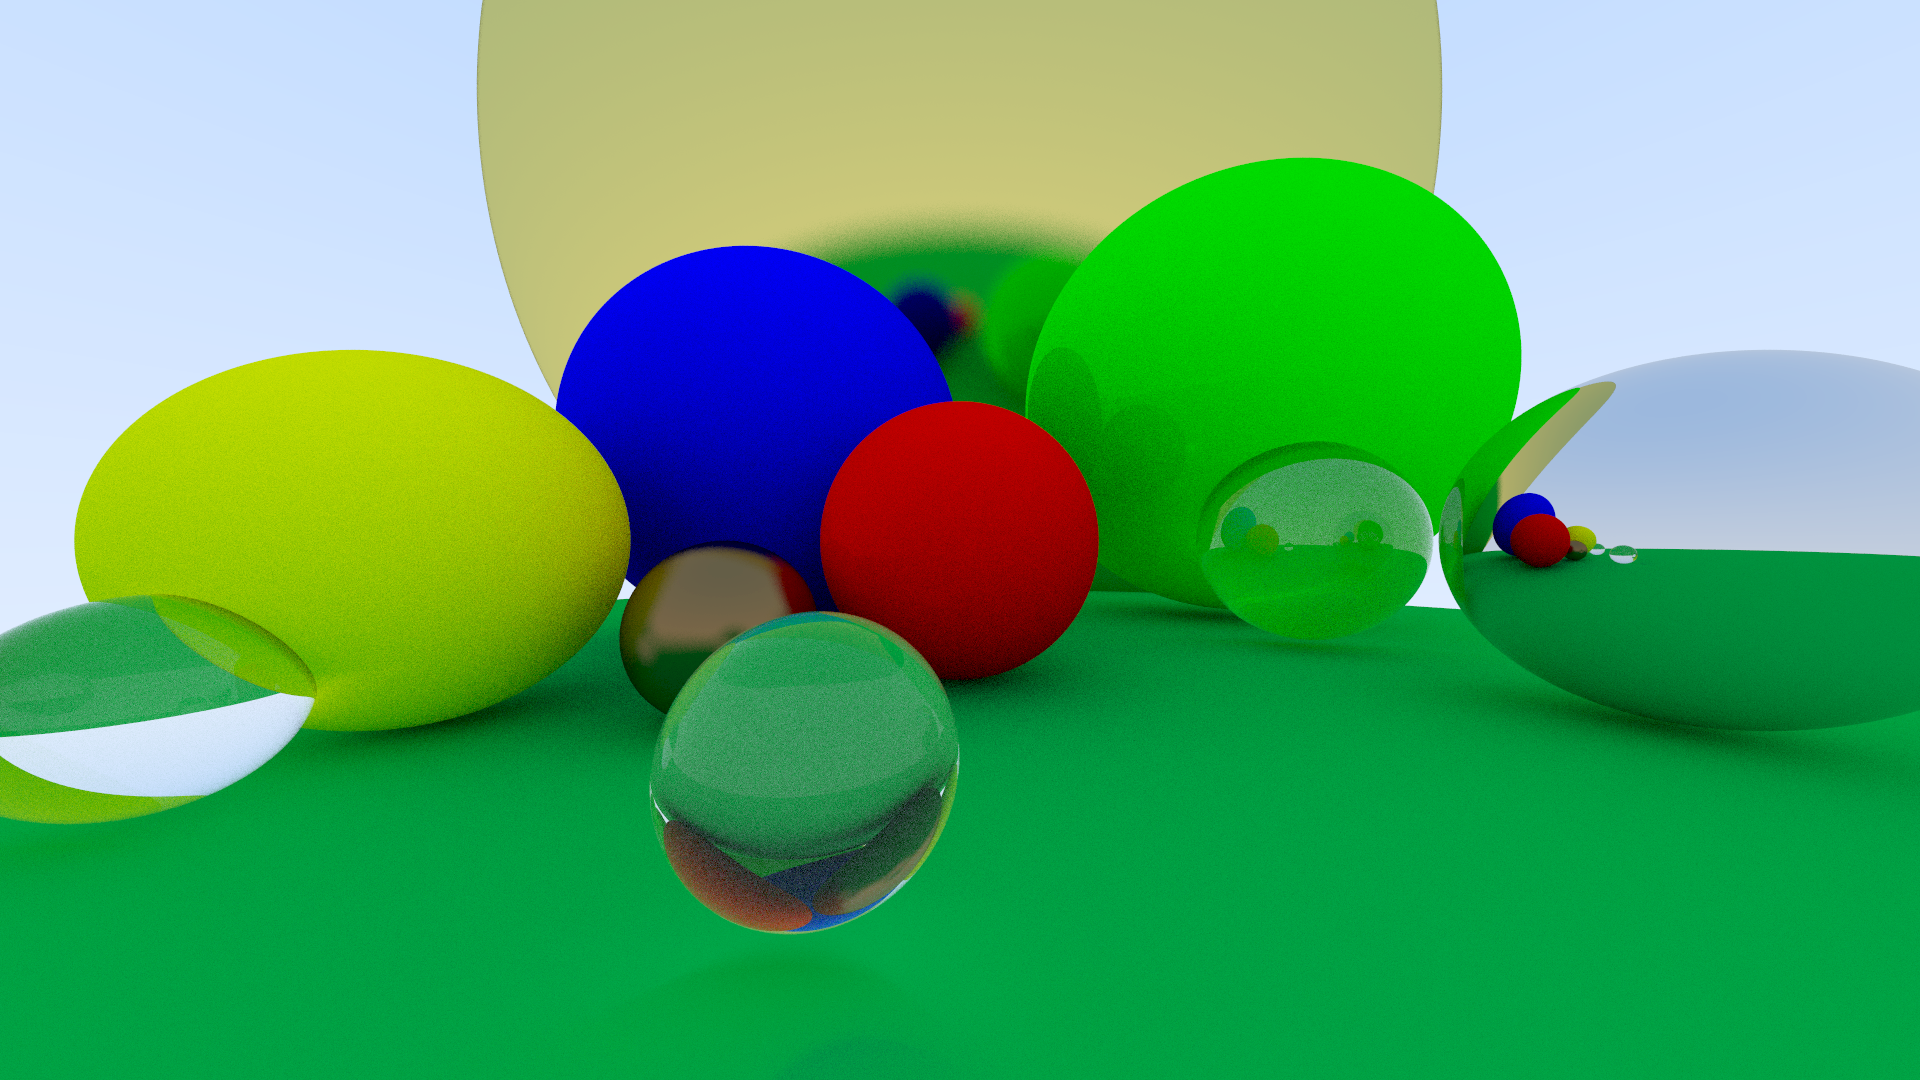
\includegraphics[width=\textwidth]{title}
\end{figure}
\begin{center}
{\Large Timo Salisch}
\end{center}
\clearpage

\tableofcontents

\newpage
\chapter{Rendering loop}
\pagenumbering{arabic}
The rendering process consists of two loops. One outer loop which iterates through the rows of the image and the inner loop iterating through the columns of the image. This way, every pixel will be visited once and the color of the pixel can be calculated. In this basic version of the rendering loop the color of every pixel will be set to (128, 64, 255). The resulting image can be seen in figure \ref{fig:step1}.
\begin{figure}[h!]

\includegraphics[width=\textwidth]{step1}
\centering
\caption{Result after running simple rendering loop}
\label{fig:step1}
\end{figure} \\
To store the already rendered information about the image, an \textit{Image} class is implemented. An instance of this class represents one image and saves the color information of every pixel using a two dimensional list. The color is represented as an instance of the \textit{Vector} class. This \textit{Vector} class saves three floating point values and offers simple arithmetic operations of (three-dimensional) vectors. These three values can either be interpreted as the world coordinates x, y and z or as the color properties red, green and blue. To change the color value of a specific pixel of the image, the \textit{Image} class provides an \textit{update} method to do so. In order for the image to be viewed, it has to be saved. The image is saved in the ''PPM'' format. This is done by the \textit{save\_image} method which expects a path and then saves the image to that path using the ''PPM'' format. For the file to be readable as ''PPM'', the first three lines have to include: ''P3'', image width and height, max color value. The actual pixel information are added by the loop iterating through the pixels. It is import to iterate through the rows beginning with the top row, otherwise the image is flipped. The saving process can be seen in source code \ref{lst:saving}.
\begin{lstlisting}[caption={Saving an image}, label=lst:saving, style=mystyle]
def save_image(self, path: str):
    image_str = f'P3\n{self.width} {self.height}\n255'
  
    for j in range(self.height)[::-1]:
        for i in range(self.width):
            red, green, blue = self.matrix[i][j].to_tuple()
            image_str = image_str + f"\n{int(red)} {int(green)} {int(blue)}"

    with open(path, mode='w+') as f:
        f.write(image_str)
\end{lstlisting}

\chapter{Camera}
jhfjgjkfgjfghjjfg

\chapter{Objects: shape}
jhfjgjkfgjfghjjfg

\chapter{Enhancing camera and rendering loop}
jhfjgjkfgjfghjjfg

\chapter{Objects material: diffuse}
jhfjgjkfgjfghjjfg

\chapter{Objects material: specular}
jhfjgjkfgjfghjjfg

\chapter{Objects material: specular transmission}
jhfjgjkfgjfghjjfg

\chapter{Lights}
jhfjgjkfgjfghjjfg

\chapter{Positioning and orienting camera}
jhfjgjkfgjfghjjfg

\chapter{Animation}
jhfjgjkfgjfghjjfg

\chapter{Render parallelization}
jhfjgjkfgjfghjjfg

\chapter{Config files}
jhfjgjkfgjfghjjfg
\end{document}